% Template LaTeX document for CSSR4Africa Deliverables
% Adapted from documents prepared by EPFL for the RobotCub project
% and subsequently by the University of Skövde for the DREAM project
%
% DV 28/06/2023

\documentclass{CSSRforAfrica}

\usepackage[hidelinks,colorlinks=false]{hyperref}
\usepackage[titletoc,title]{appendix}
\usepackage{latexsym}
\usepackage{xcolor}
\usepackage{dirtree}
\usepackage{natbib} 
\usepackage{tikz}
\usepackage{listings}
\usepackage{amsmath}
\usetikzlibrary{shapes.geometric, arrows, positioning, fit}
\newcommand{\blank}{~\\}
\newcommand{\checkbox}{{~~~~~~~\leavevmode \put(-7,-1.5){  \huge $\Box$  }}}

\begin{document}
\input{epsf}

%%
%% SHOULD NOT NEED TO BE CHANGED BEFORE THIS POINT
%% ------------------------------------------------
%%

\deliverable{D5.5.2.1}          
\title{D.5.5.2.1 English Text to Speech Conversion.}   

\leadpartner{Carnegie Mellon University Africa }    
\partner{}                                % INSERT partner name: Carnegie Mellon University Africa or The University of the Witwatersrand

\revision{1.2}                         
\deliverabledate{26/02/2025}  
\submissiondate{02/03/2025} 
\revisiondate{23/04/2025}       
\disseminationlevel{PU}
\responsible{Richard Muhirwa }       


%%
%% Create the titlepage
%%

\maketitle
 

\section*{Executive Summary}
Deliverable D5.5.2.1 presents the outcomes of implementing English Text-to-Speech (TTS) functionality on the Pepper robot platform. This document outlines the results of each stage of the software development process, covering requirements definition, module design, testing, and implementation.

The English Text to Speech conversion function enables the Pepper robot to transform written text into spoken words through its internal speakers. This capability is fundamental to the robot's ability to verbally communicate with users, supporting a wide range of interactions from basic greetings to complex information delivery\cite{Bartnecketal2020}. The system accepts text input via ROS messages on the \texttt{/speech} topic and processes this text through the NAOqi ALTextToSpeech engine.

This report outlines the functional requirements, interface design specifications, module architecture, testing approach, and implementation instructions for the Text to Speech conversion system. Testing results confirm that the Pepper robot's TTS system through the ROS interface functions correctly, producing clear, intelligible speech for a wide range of inputs, and maintaining stability even under stress conditions.


%===============================================================
\label{executive_summary}
%%\addcontentsline{toc}{section}{Executive Summary}
 

\newpage
 
 
%\graphicspath{{./figs/}}
\pagebreak
\tableofcontents
\newpage


\section{Introduction}
%===============================================================
Text to Speech (TTS) conversion is a critical component of human-robot interaction systems, enabling robots to communicate verbally with human users. In the context of the Pepper robot platform, the TTS function serves as the auditory output mechanism that allows the robot to deliver information, respond to queries, and engage in natural-sounding dialogue.
The TTS conversion process follows a sequence of operations: text is received as input, processed through language-specific rules for pronunciation and intonation, and then synthesized as audio output\cite{Zen2009}. This process requires consideration of various linguistic features such as sentence structure, punctuation, abbreviations, and special characters to produce speech that sounds natural. \\

Within the Pepper robot system, the TTS function receives text input through the Robot Operating System (ROS) messaging framework and utilizes the NAOqi ALTextToSpeech engine for the actual speech synthesis. This architecture allows for standardized communication between different system components while leveraging the optimized speech synthesis capabilities built into the robot's native software platform.

\begin{figure}[h]
    \centering
    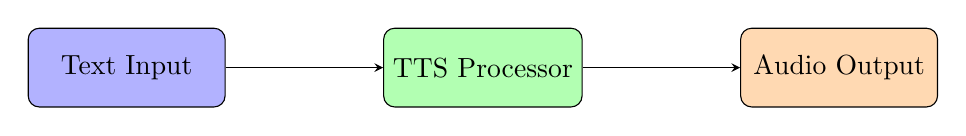
\begin{tikzpicture}[node distance=2cm]
        \node[draw, fill=blue!30, rounded corners, minimum width=2.5cm, minimum height=1cm] (input) {Text Input};
        \node[draw, fill=green!30, rounded corners, minimum width=2.5cm, minimum height=1cm, right=of input] (processor) {TTS Processor};
        \node[draw, fill=orange!30, rounded corners, minimum width=2.5cm, minimum height=1cm, right=of processor] (output) {Audio Output};
        
        \draw[-stealth] (input) -- (processor);
        \draw[-stealth] (processor) -- (output);
    \end{tikzpicture}
    \caption{Basic workflow of a Text-to-Speech system.}
    \label{fig:tts-workflow}
\end{figure}

%\cite{Bartnecketal2020}; 

 
\newpage
\section{ Requirements definition}
%===============================================================
The English Text to Speech (TTS) conversion function is required to convert text input into audible speech output on the Pepper robot. The function must accept English text input in various formats including sentences, paragraphs, and questions. It needs to process special characters, numbers, dates, and abbreviations correctly, ensuring proper pronunciation of these elements in the resulting speech.
The system should produce natural-sounding speech with appropriate intonation, conveying the meaning and intent of the original text. Various speech parameters, including speed, volume, and pitch, should be supported if the underlying engine allows for such customization, providing flexibility in speech delivery. However, these parameters are not supported in the ROS configuration. \\
The text-to-speech conversion process follows a straightforward flow from text input to speech output, with several key requirements governing this transformation, as illustrated in Figure~\ref{fig:tts-requirements}.

\begin{figure}[htbp]
    \centering
    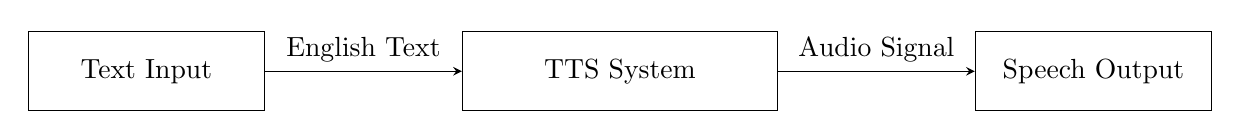
\begin{tikzpicture}[node distance=2.5cm]
    \usetikzlibrary{positioning, calc, arrows.meta}
        % Define blocks
        \node (text) [rectangle, draw, minimum width=3cm, minimum height=1cm] {Text Input};
        \node (tts) [rectangle, draw, minimum width=4cm, minimum height=1cm, right=of text] {TTS System};
        \node (speech) [rectangle, draw, minimum width=3cm, minimum height=1cm, right=of tts] {Speech Output};
        
        % Draw arrows
        \draw[-stealth] (text) -- (tts) node[midway, above] { English Text };
        \draw[-stealth] (tts) -- (speech) node[midway, above] { Audio Signal };
        
    \end{tikzpicture}
    \caption{Text-to-Speech Conversion Requirements Overview}
    \label{fig:tts-requirements}
\end{figure}

The system should produce natural-sounding speech with appropriate intonation, conveying the meaning and intent of the original text.
The TTS function must operate reliably for both short phrases and longer text passages, ensuring consistent performance regardless of input length. Consistent performance across multiple invocations is essential, with the system maintaining the same quality standards each time it is used. The system must maintain responsiveness even with rapid successive requests, handling a queue of speech tasks efficiently.\\
These requirements collectively ensure that the TTS function provides a robust and natural voice communication channel for the Pepper robot. \\


\newpage
\section{Function specification}
%===============================================================

The TTS function transforms text strings into audible speech through a specific process flow. Initially, the function receives text input via ROS message on the /speech topic. This message contains the string data to be spoken by the robot. The function then parses and normalizes the text, handling punctuation, abbreviations, and numbers according to English language rules.\\
After normalization, the text is processed through the NAOqi ALTextToSpeech engine, which converts the text into an audio stream using the appropriate voice synthesis algorithms. Finally, the system generates audio output through the robot's speakers, producing the audible speech corresponding to the input text.

The TTS function transforms text strings into audible speech through a specific process flow, as shown in Figure~\ref{fig:tts-dataflow}. This multi-stage pipeline ensures proper handling of text at each step.

\usetikzlibrary{positioning, calc, arrows.meta}
\begin{figure}[htbp]
    \centering
    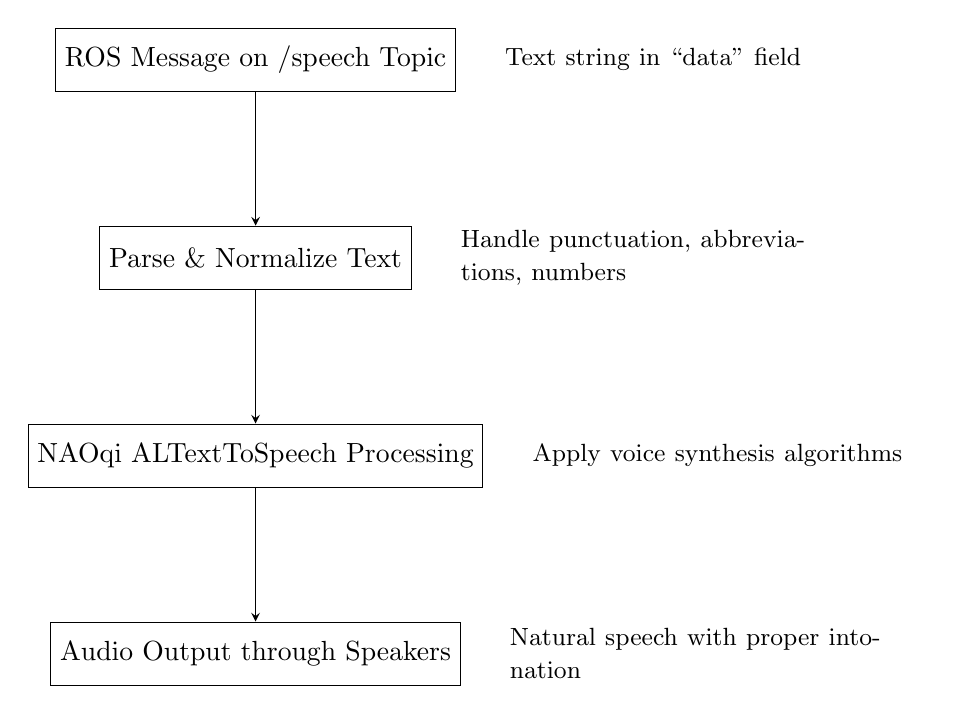
\begin{tikzpicture}[node distance=1.7cm]
   % \usetikzlibrary{positioning, calc, arrows.meta}
        % Define nodes
        \node (input) [rectangle, draw, minimum width=3cm, minimum height=0.8cm] {ROS Message on /speech Topic};
        \node (parse) [rectangle, draw, minimum width=3cm, minimum height=0.8cm, below=of input] {Parse \& Normalize Text};
        \node (process) [rectangle, draw, minimum width=3cm, minimum height=0.8cm, below=of parse] {NAOqi ALTextToSpeech Processing};
        \node (output) [rectangle, draw, minimum width=3cm, minimum height=0.8cm, below=of process] {Audio Output through Speakers};
        
        % Draw arrows
        \draw[-stealth] (input) -- (parse);
        \draw[-stealth] (parse) -- (process);
        \draw[-stealth] (process) -- (output);
        
        % Add data descriptions
        \node[right=0.5cm of input, text width=5cm] {\small Text string in ``data" field};
        \node[right=0.5cm of parse, text width=5cm] {\small Handle punctuation, abbreviations, numbers};
        \node[right=0.5cm of process, text width=5cm] {\small Apply voice synthesis algorithms};
        \node[right=0.5cm of output, text width=5cm] {\small Natural speech with proper intonation};
    \end{tikzpicture}
    \caption{Text-to-Speech Data Transformation Flow}
    \label{fig:tts-dataflow}
\end{figure}


The expected input data for the TTS function consists of text strings in English language, which may include various formats such as statements, questions, and commands. The input may contain special characters and punctuation marks that influence the speech pattern, as well as numbers, dates, times, and abbreviations that require special parsing rules. Text length can range from single words to multiple paragraphs, with the system handling all lengths appropriately.\\
For output, the function produces audible speech through the robot's speakers with several key characteristics. The speech should have a natural-sounding voice with appropriate intonation patterns. Words, numbers, and abbreviations should be pronounced correctly according to English language rules. The speech should have proper pacing with appropriate pauses at punctuation marks, simulating natural human speech patterns.


\newpage
\section{Interface design}
%===============================================================
\subsection{Directory Structure}

The englishTTS model for testing its functionality follows this directory structure:

\vspace{1cm}
\dirtree{%
.1 cssr4africa/.
.2 unit\_test/.
.3 src/.
.4 english\_tts\_test/.
.5 english\_tts\_test.py.
.5 README.md.
.3 CMakeLists.txt.
.3 package.xml.
.2 cssr\_system/.
.3 ....
}
\vspace{1cm}

\subsection{Input Data Specification}
The function receives data via a ROS message on the \texttt{/speech} topic. The message type used is \texttt{std\_msgs/String}, which contains a data field of type string. This field contains the text to be spoken by the robot. An example command for publishing a message to this topic would be: \texttt{rostopic pub /speech std\_msgs/String "data: 'Hello world'"}. This standardized interface ensures compatibility with other ROS-based components in the system.
\subsection{Output Data Specification}
The function outputs audio through the robot's speakers without returning data to the ROS system. The output is purely auditory, with no programmatic feedback provided by default. Future enhancements could include additional output data such as completion notification messages, speech status updates during processing, and error reporting for failed speech attempts. These enhancements would provide better monitoring and error handling capabilities for the system.
\subsection{Test Driver Specification}
The test driver for this system connects to the ROS network and generates test text inputs from predefined sets or parameter files. It publishes these test messages to the \texttt{/speech} topic and waits for appropriate intervals between tests to avoid overlapping speech output. The driver logs test execution for later analysis.
Test data is sourced from the Robot Behavior Specification, including basic greetings and interactions, information delivery statements, questions and responses, and complex narrative passages. This comprehensive test set ensures that all aspects of the TTS function are evaluated under realistic usage conditions.


\newpage
\section{Module design}
%===============================================================

\subsection{Algorithms and Data Structures}

 The ROS Subscriber/Publisher communication method is used for message handling, providing a standardized communication framework. The NAOqi ALTextToSpeech API is used for speech synthesis, leveraging the built-in capabilities of the Pepper robot platform.
A simple queue data structure manages multiple speech requests, ensuring they are processed in order without overlapping. Text normalization algorithms handle numbers, dates, and abbreviations, converting them into forms that can be properly vocalized by the speech synthesis engine.


\subsection{Technology Selection}

After investigation, NAOqi ALTextToSpeech through the ROS interface (naoqi\_driver package) was selected as the primary technology for speech synthesis. This approach leverages the optimized native speech capabilities of the Pepper robot while maintaining compatibility with the ROS-based system architecture.
Standard ROS messaging is used for communication between components, providing a well-established framework for distributed robotics applications. Python was chosen as the implementation language due to its compatibility with both ROS and NAOqi, as well as its rich ecosystem of text processing libraries.


\subsection{Coding Implementation}

To run the English TTS functionality, users must first navigate to the root of their ROS workspace and build the project using the \texttt{catkin\_make} command, followed by sourcing the development setup script with \texttt{source devel/setup.bash}.
To launch the system, the naoqi driver must be started first with the command: \\
\texttt{roslaunch naoqi\_driver naoqi\_driver.launch \newline nao\_ip:=172.29.111.230 network\_interface:=enp0s3}. \\ This establishes the connection to the robot's internal systems.
Once the driver is running, the TTS node can be launched in a separate terminal with: 
\texttt{source devel/setup.bash} followed by \texttt{rostopic pub /text to say std msgs/string "data: 'Hello World.'"}. This command sends a text string to the system, which will then be converted to speech output on the robot.     



\newpage
%===============================================================

\section{User Manual}

\subsection{Building the System}

To run the English TTS functionality, follow these detailed steps:


% Define colors
\definecolor{commentgreen}{RGB}{0, 155, 0}
\definecolor{backgroundcolor}{RGB}{240, 240, 249}
\definecolor{codeblack}{RGB}{0, 0, 0}
% \definecolor{stringblue}{RGB}{255, 165, 0}

% Configure listing style
\lstdefinestyle{commandstyle}{
  backgroundcolor=\color{backgroundcolor},
  basicstyle=\ttfamily\color{codeblack}\footnotesize,
  commentstyle=\color{commentgreen},
  % stringstyle=\color{stringblue},
  numbers=none,
  breaklines=true,
  breakatwhitespace=true,
  tabsize=2,
  showspaces=false,
  showstringspaces=false,
  frame=single,
  framesep=3pt,
  xleftmargin=5pt,
  xrightmargin=5pt,
  framexleftmargin=5pt,
  framexrightmargin=5pt,
  framextopmargin=3pt,
  framexbottommargin=3pt,
  framerule=0pt,
  % The important addition:
  morecomment=[l]{\#},  % This tells LaTeX that lines starting with # are comments
 morestring=[b]',      % Single-quoted strings
 morestring=[b]"       % Double-quoted strings
}


\begin{enumerate}
    \item First, navigate to the root directory of your ROS workspace using the terminal. This is the main directory that contains your \texttt{src}, \texttt{build}, and \texttt{devel} folders. For example: \texttt{cd \textasciitilde/catkin\_ws}

    \item Build all packages in your workspace using the \texttt{catkin\_make} command. This compiles all the necessary code and creates executable files:
    \begin{lstlisting}[style=commandstyle]
    catkin_make
    \end{lstlisting}
    This process might take several minutes depending on the size of your workspace and the speed of your computer. The command will display compilation messages, and should end with a success message if everything is built correctly.

    \item After the build completes successfully, you need to source the setup script to ensure that the ROS environment recognizes your newly built packages:
    \begin{lstlisting}[style=commandstyle]
    source devel/setup.bash
    \end{lstlisting}

    This command adds your workspace packages to the ROS package path, making them available for use.
\end{enumerate}

\subsection{Launching the NAOqi Driver}

Before using the TTS functionality, you must establish a connection with the Pepper robot by launching the NAOqi driver:

\begin{enumerate}
    \item Launch the NAOqi driver with the following command:
    \begin{lstlisting}[style=commandstyle]
    roslaunch naoqi_driver naoqi_driver.launch nao_ip:=172.29.111.230 network_interface:=enp0s3
    \end{lstlisting}
    
    The parameters in this command have the following meanings:
    \begin{itemize}
        \item \texttt{nao\_ip}: Specifies the IP address of the Pepper robot (replace with your robot's actual IP if different)
        \item \texttt{network\_interface}: Specifies which network interface on your computer to use for the connection (replace \texttt{enp0s3} with your computer's network interface if different)
    \end{itemize}

    \item After running this command, you should see a series of initialization messages as the driver establishes a connection with the robot. Wait until you see messages indicating that the connection is successfully established and the driver is running.
\end{enumerate}

\subsection{Using the Text-to-Speech Functionality}

Once the NAOqi driver is running, you can use the TTS functionality by following these steps:

\begin{enumerate}
    \item Open a new terminal tab or window (while keeping the NAOqi driver running in the previous terminal).

    \item In the new terminal, source the setup script again to ensure the ROS environment is properly configured:
    \begin{lstlisting}[style=commandstyle]
    source devel/setup.bash
    \end{lstlisting}

    \item To make the robot speak, publish a message to the \texttt{/speech} topic using the \texttt{rostopic} command:
    \begin{lstlisting}[style=commandstyle]
    rostopic pub /speech std_msgs/String "data: 'Hello World.'"
    \end{lstlisting}
    
    This command has the following components:
    \begin{itemize}
        \item \texttt{rostopic pub}: The ROS command for publishing a message to a topic
        \item \texttt{/speech}: The name of the topic that the TTS system is listening to
        \item \texttt{std\_msgs/String}: The message type (a standard string message)
        \item \texttt{"data: 'Hello World.'"}: The actual message content, where 'Hello World.' is the text that will be spoken
    \end{itemize}

    \item Upon receiving this message, the TTS system will process the text and the Pepper robot will speak the words "Hello World" through its speakers.
\end{enumerate}


\subsection{Troubleshooting}

If the robot does not speak after publishing a message, check the following:

\begin{enumerate}
    \item Ensure the NAOqi driver is running correctly and shows no error messages
    \item Verify that you're publishing to the correct topic name
    \item Check that the robot's volume is turned up
    \item Confirm that the robot's IP address is correct in the launch command
    \item Check the ROS logs for any error messages using the command: \texttt{roscd log}
\end{enumerate}

If problems persist, try restarting both the NAOqi driver and the robot itself.

\newpage


%===============================================================
\newpage
\section{Testing Report}

The Text-to-Speech system underwent rigorous testing to ensure correct functionality across various scenarios and input types. Both automated unit tests and interactive functional tests were conducted to validate the system's performance.

\subsection{Unit Testing Results}

The tests were designed to verify basic speech functionality, sentence handling, special character processing, question intonation, and multi-sentence capabilities. The following command was used to execute the unit tests:

\begin{lstlisting}[style=commandstyle]
# Make sure the robot is running
# In a new terminal:
rosrun unit_test english_tts_test.py
\end{lstlisting}


This test suite performed a series of interactive tests that required human verification of the speech output. The tests included:

\begin{lstlisting}[style=commandstyle]
==================================================================
ENGLISH TTS TEST
==================================================================
...........................
TEST: Basic Speech
...........................
Speaking: "Hello world"
Waiting 3 seconds for speech to complete...
...
Did you hear the robot speak? (y/n): y
 Test passed! Robot spoke successfully.

...........................
TEST: Longer Sentence
...........................
Speaking: "This is a longer sentence to test the Text to Speech system on the robot."
Waiting 5 seconds for speech to complete...
.....
Did you hear the robot speak? (y/n): y
 Test passed! Robot spoke successfully.

...........................
TEST: Special Characters
...........................
Speaking: "Testing with numbers 1, 2, 3 and punctuation!"
Waiting 3 seconds for speech to complete...
...
Did you hear the robot speak? (y/n): y
 Test passed! Robot spoke successfully.

...........................
TEST: Question Intonation
...........................
Speaking: "Is this working correctly? I hope so."
Waiting 4 seconds for speech to complete...
....
Did you hear the robot speak? (y/n): y
 Test passed! Robot spoke successfully.

...........................
TEST: Multiple Sentences
...........................
Speaking: "First sentence. Second sentence. Third sentence."
Waiting 5 seconds for speech to complete...
.....
Did you hear the robot speak? (y/n): y
 Test passed! Robot spoke successfully.

==================================================================
TEST SUMMARY
==================================================================
Basic Speech: PASSED
Longer Sentence: PASSED
Special Characters: PASSED
Question Intonation: PASSED
Multiple Sentences: PASSED

5/5 tests passed (100.0%)

All tests passed successfully!
\end{lstlisting}


These functional tests confirm that the TTS system correctly handles various text inputs and produces appropriate speech output. The human verification component was essential for assessing the quality aspects that cannot be automatically measured, such as natural intonation, correct pronunciation, and overall intelligibility.

\subsection{Comprehensive Testing Analysis}

By running interactive functional unit tests, we were able to evaluate both the technical integration and the user-perceived quality of the TTS system. The tests demonstrated that:

\begin{enumerate}
    \item The system correctly interfaces with ROS messaging
    \item Basic and complex sentences are processed correctly
    \item Special characters and numbers are pronounced appropriately
    \item Question intonation is properly applied
    \item Multiple sentences are handled with correct pacing and pauses
\end{enumerate}

The manual verification approach for functional tests was necessary due to the subjective nature of speech quality assessment. Aspects such as naturalness, proper intonation, and overall intelligibility require human judgment to evaluate effectively.

\newpage
\bibliographystyle{unsrt}
%================================================================


\bibliography{cognitive_systems.bib}                                     % REPLACE with correct filename
\addcontentsline{toc}{section}{References}



\pagebreak
\section*{Principal Contributors}
%===============================================================
\label{contributors}
\addcontentsline{toc}{section}{Principal Contributors}
The main authors of this deliverable are as follows (in alphabetical order).
\blank
~
\blank
David Vernon, Carnegie Mellon University Africa.\\    % REPLACE with correct name and affiliation
Richard Muhirwa, Carnegie Mellon University Africa.\\    % REPLACE with correct name and affiliation
                                                                        

% ================================================================
\newpage

\section*{Document History}
%================================================================
\addcontentsline{toc}{section}{Document History}

\label{document_history}

\begin{description}

\item [Version 1.0]~\\
First draft. \\
Richard  Muhirwa. \\            
02 March 2025.               

\item [Version 1.1]~\\
I updated the unit testing section to reflect the current software implementation. \\
Updated Figure 2 to make it more readable. 
Removed ambious terminology "utilizes several key technologies" in section 5 Module design.\\
Richard Muhirwa \\
16 April 2025

\item [Version 1.2]~\\
Update Interface design subsection Directory structure.\\
Formatted all commands as codes with light gray background.\\
Richard  Muhirwa. \\                                     
23 April 2025.

\end{description}

\end{document}

